\documentclass[a4paper,12pt]{article}

\usepackage{amsmath,amssymb,multicol,tikz,enumitem}
\usepackage[margin=2cm]{geometry}
\usetikzlibrary{calc,shapes}

\pagestyle{empty}

\newcommand\N{\mathbf{N}}
\newcommand\Q{\mathbf{Q}}
\newcommand\R{\mathbf{R}}
\newcommand\Z{\mathbf{Z}}

\usepackage{array}
\newcolumntype{P}[1]{>{\centering\arraybackslash}p{#1}}
\newcommand\indd{${}$\hspace{20pt}}

\begin{document}

\begin{center}
\parbox{3.5cm}{\textbf{Data Structures}} \hfill {\bf\Huge Worksheet 5} \hfill \parbox{3.5cm}{\flushright\textbf{BITL2}} \\[5pt]
\rm\small 14 October 2021
\end{center}

\hrule\vspace{2pt}\hrule


\vspace{10pt}
\noindent
This worksheet uses the following definitions.
\begin{itemize}
\item \textbf{height of a node:} length of the longest path from a node to a leaf below it
\item \textbf{height-balanced (AVL) tree}: satisfies $|$height$($right child$)-$height$($left child$)| \leqslant 1$
\end{itemize}
\hrule


\begin{enumerate}

\item \textbf{Warm up:} Answer the following questions about tree structures.`
\begin{enumerate}
\item What is the shortest and longest path between two level $\ell$ nodes in a binary tree?
\item What is the smallest and largest numbers of leaves a height $h$ binary tree can have?
\item What is the heap property of a tree?
\item What is the advantage of using heaps for sorting?
\end{enumerate}

\vfill
\item In the \textbf{max-heap} below left, perform the operations below right, in the given order.
\[
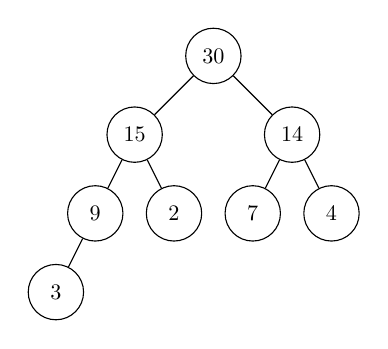
\begin{tikzpicture}[baseline=1.5cm]
\foreach \x\y\n\l in {.5/0/a/3, 1/1/b/9, 2/1/c/2, 3/1/d/7, 4/1/e/4, 1.5/2/f/15, 3.5/2/g/14, 2.5/3/h/30}{
  \node[circle,draw,minimum size=25pt,scale=.8] (\n) at (\x,\y) {\l};
}
\foreach \x\y in {a/b, b/f, c/f, d/g, e/g, f/h, g/h}{
  \draw (\x)--(\y);
}
\end{tikzpicture}
\hspace{2cm}
\begin{array}{l}
\text{(a) insert 16} \\[5pt]
\text{(b) insert 17} \\[5pt]
\text{(c) remove max} \\[5pt]
\text{(d) insert 18} \\[5pt]
\text{(e) insert 19}
\end{array}
\]
\begin{enumerate}\setcounter{enumii}{5}
\item Give the 0-based array that stores the heap after the steps above have been applied.
\end{enumerate}

\vfill
\item In the \textbf{binary search tree} below left, perform the operations below right, in the given order. For each insert operation, show the path taken when searching for the spot to insert the key.
\[
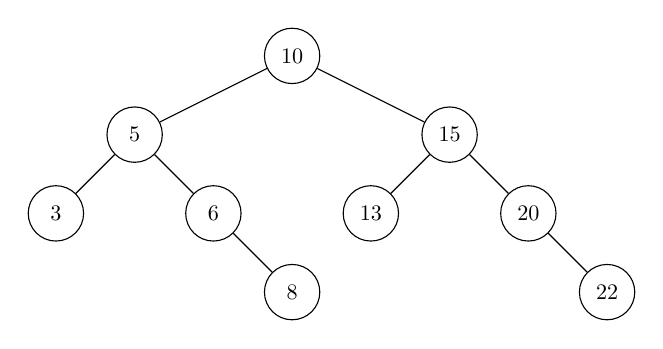
\begin{tikzpicture}[baseline=1.5cm]
\foreach \x\y\n\l in {3/0/a/8, 7/0/b/22, 0/1/c/3, 2/1/d/6, 4/1/e/13, 6/1/f/20, 1/2/g/5, 5/2/h/15, 3/3/i/10}{
  \node[circle,draw,minimum size=25pt,scale=.8] (\n) at (\x,\y) {\l};
}
\foreach \x\y in {a/d, b/f, c/g, d/g, e/h, f/h, g/i, h/i}{
  \draw (\x)--(\y);
}
\end{tikzpicture}
\hspace{2cm}
\begin{array}{l}
\text{(a) insert 7} \\[5pt]
\text{(b) insert 14} \\[5pt]
\text{(c) delete 15} \\[5pt]
\text{(d) insert 15} \\[5pt]
\text{(e) delete 10} \\[5pt]
\text{(f) insert 10} 
\end{array}
\]
\begin{enumerate}\setcounter{enumii}{6}
\item Give the DFS postorder of the tree after the steps above have been applied.
\end{enumerate}

\vfill
\clearpage
\item In the \textbf{AVL tree} below left, perform the operations below right, in the given order. Make sure to rebalance (if necessary) after every operation.
\[
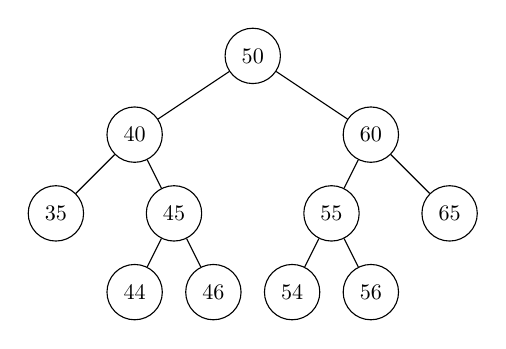
\begin{tikzpicture}[baseline=2.5cm]
\foreach \x\y\n\l in {2/1/a/44, 3/1/b/46, 4/1/c/54, 5/1/d/56, 1/2/e/35, 2.5/2/f/45, 4.5/2/g/55, 6/2/h/65, 2/3/i/40, 5/3/j/60, 3.5/4/k/50}{
  \node[circle,draw,minimum size=25pt,scale=.8] (\n) at (\x,\y) {\l};
}
\foreach \x\y in {a/f, b/f, c/g, d/g, e/i, f/i, g/j, h/j, i/k, j/k}{
  \draw (\x)--(\y);
}
\end{tikzpicture}
\hspace{2cm}
\begin{array}{l}
\text{(a) insert 43} \\[5pt]
\text{(b) insert 66} \\[5pt]
\text{(c) insert 67} \\[5pt]
\text{(d) remove 60} \\[5pt]
\end{array}
\]
Recall that rebalancing is done in terms of \textbf{rotations}.  The \textbf{$x$-over-$y$} rotation of $T$, for nodes $x,y$ of $T$ where $x$ is a child of $y$, is a new tree $T'$ identical to $T$, except for:
\begin{itemize}
\item if $T.y.parent=z$, then $T'.x.parent = z$ and  $T'.y.parent=x$
\item if $T.y.leftchild=x$, then $T'.y.leftchild = T.x.rightchild$
\item if $T.y.rightchild=x$, then $T'.y.rightchild = T.x.leftchild$
\end{itemize}

%\vspace{1cm}

%\item

\end{enumerate}

\end{document}